\documentclass[conference]{IEEEtran}
\IEEEoverridecommandlockouts
% The preceding line is only needed to identify funding in the first footnote. If that is unneeded, please comment it out.
\usepackage{cite}
\usepackage{amsmath,amssymb,amsfonts}
\usepackage{algorithmic}
\usepackage{graphicx}
\usepackage{textcomp}
\usepackage{xcolor}
\usepackage{hyperref}

\def\BibTeX{{\rm B\kern-.05em{\sc i\kern-.025em b}\kern-.08em
    T\kern-.1667em\lower.7ex\hbox{E}\kern-.125emX}}
\begin{document}

\title{PETRAS: \textbf{P}arameter \textbf{E}fficient finetuning of Image \textbf{Tra}nsformers for \textbf{S}egmentation}

\author{\IEEEauthorblockN{Neel Gupta}
\IEEEauthorblockA{\textit{School of Computer Science} \\
\textit{University College Cork}\\
College Rd, Cork, Ireland \\
neelgupta04@outlook.com}}

\maketitle

\begin{abstract}
This technical report presents our approach submitted to the UCC AI Quest competition, addressing challenges of low-quality data, noisy labels, and limited diversity. We propose a method for parameter-efficient fine-tuning of a large foundation model on consumer hardware, utilizing cutting-edge innovations. Our model exhibits robustness, generalization to unseen data, and proficient handling of edge cases. All associated code \& materials shall be released publicly on GitHub under a permissive license.
\end{abstract}

\begin{IEEEkeywords}
Deep learning, Transfer Learning, Pre-Trained Model, Fine-Tuning, Image Segmentation
\end{IEEEkeywords}

\section{Introduction}
In this report, we outline our attempt at the UCC AI Quest competition, wherein the task is to build an end-to-end pipeline to consume aerial photographs and "recognise vegetation patches in Irish natural places". \newline \break
We leverage pretrained foundation models released by MetaAI and fine-tune them in a parameter efficient way to handle the noisy datapoints and gurantee strong O.O.D (Out of distribution) generalization.
\section{The Team}

\subsection{Team Leader - Neel Gupta}

Neel is a 1\textsuperscript{st} year Data Science \& Analytics student. He is very interested in AI research and has worked in collaboration with organizations such as \href{https://stability.ai/research}{Stability AI} and \href{https://comma.ai}{Comma AI}, as well as an internship at \href{https://www.techireland.org/companies/andrson}{Andrson} - an Irish startup focused on blending music with Generative AI. He is currently working on extending Universal Transformers \cite{b1, b2} for adaptive computation and has secured research grants from Algovera AI as well as Google's TPU Research Cloud (\href{https://sites.research.google/trc/about/}{TRC}) to support his research.

\section{Related Work}

\begin{figure}
    \centering
    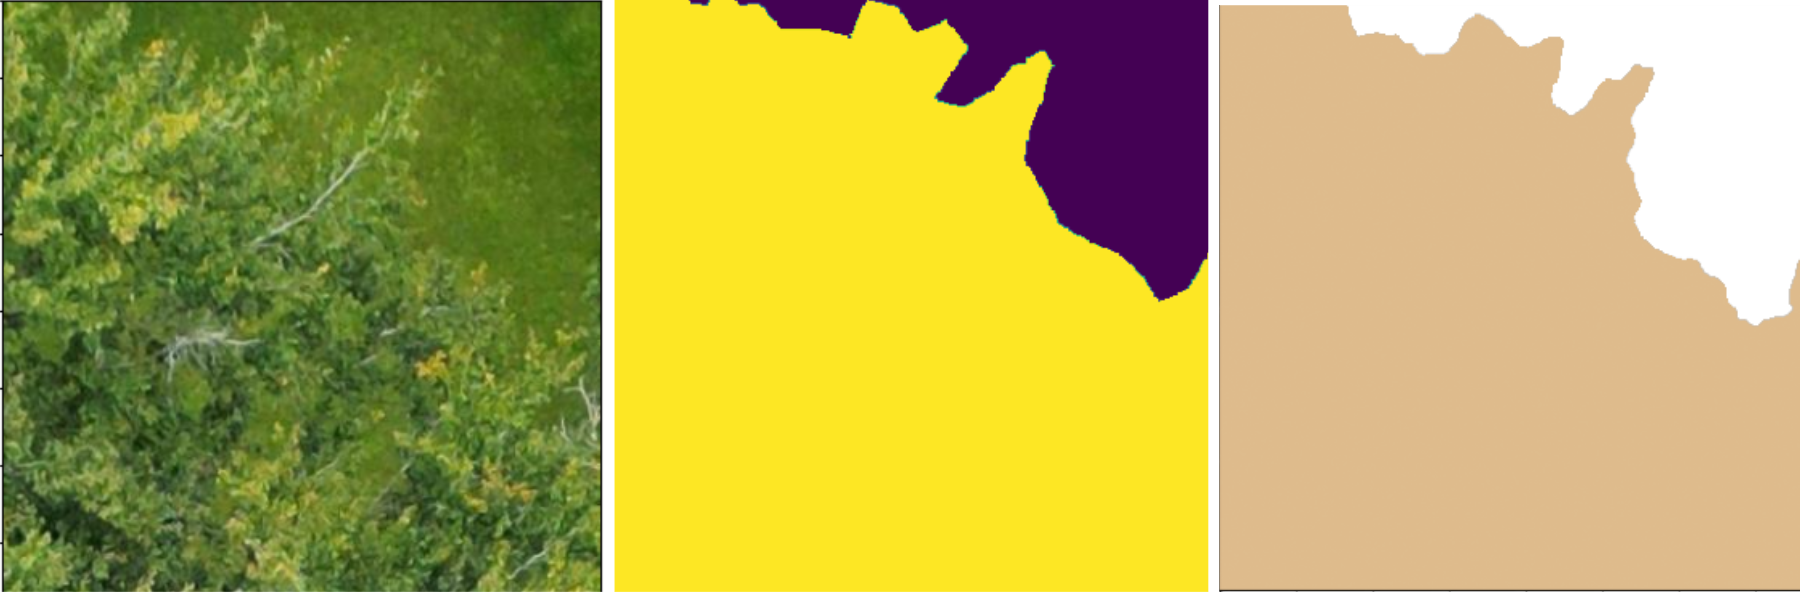
\includegraphics[width=1.1\linewidth]{cropped_model_pred.png}
    \caption{An example visualization from the validation set. i) The original image, ii) The provided (noisy) mask annotation iii) Our method}
    \label{fig:enter-label}
\end{figure}

In recent years, the proliferation of neural networks has significantly impacted various domains, catalyzed by groundbreaking methodologies such as Convolutional Neural Networks (CNNs) \cite{b3, b4} and Recurrent Neural Networks (RNNs) \cite{b5}. While these approaches have demonstrated remarkable success on small-scale datasets, challenges arise when scaling due to issues such as gradient flow instability in RNNs \cite{b6} and the limited parallelizability inherent in traditional architectures \cite{b7, b8}.
\\

The advent of self-attention mechanisms, as pioneered by Vaswani et al. \cite{b9}, represents a pivotal advancement in addressing these challenges. By enabling models to selectively attend to relevant information and capture long-range dependencies \cite{b10}, self-attention has substantially enhanced scalability \cite{b11}. Consequently, architectures leveraging self-attention, notably Vision Transformers (ViTs) \cite{b13}, have emerged as state-of-the-art solutions in computer vision tasks, leveraging their inherent flexibility and reduced inductive biases.\\

A notable development in this trajectory is the rise of generalist foundation models exemplified by Meta's SAM (Segment Anything) \cite{b14}. Pretrained on vast datasets, these models exhibit remarkable sample efficiency when adapted to domain-specific tasks, offering substantial computational savings while delivering robust and generalizable performance \cite{b15}.

\section{Approach}
\subsection{Base Architecture}
In our endeavor for computational efficiency and leveraging prior knowledge encoded in pretrained foundation models, we adopted PeFT (Parameter-efficient Fine-tuning) \cite{b16} as opposed to vanilla In-context learning. PeFT offers an efficient alternative to a full finetune, extracting maximum performance and integrating domain-specific priors while being computationally light.

Our approach utilizes the base SAM model, built upon the ViT-base flavour mentioned earlier. This variant comprises of 75 million trainable parameters. Notably, we depart from the conventional practice of freezing the encoder and training only the decoder - Instead, we opt to train the entire model end-to-end. This is rooted in both empirical observations and theoretical considerations, as we hypothesize that our task stands to benefit from relying on finer-grained domain-specific features to obtain a better encoding of the image.

\begin{figure}
    \centering
    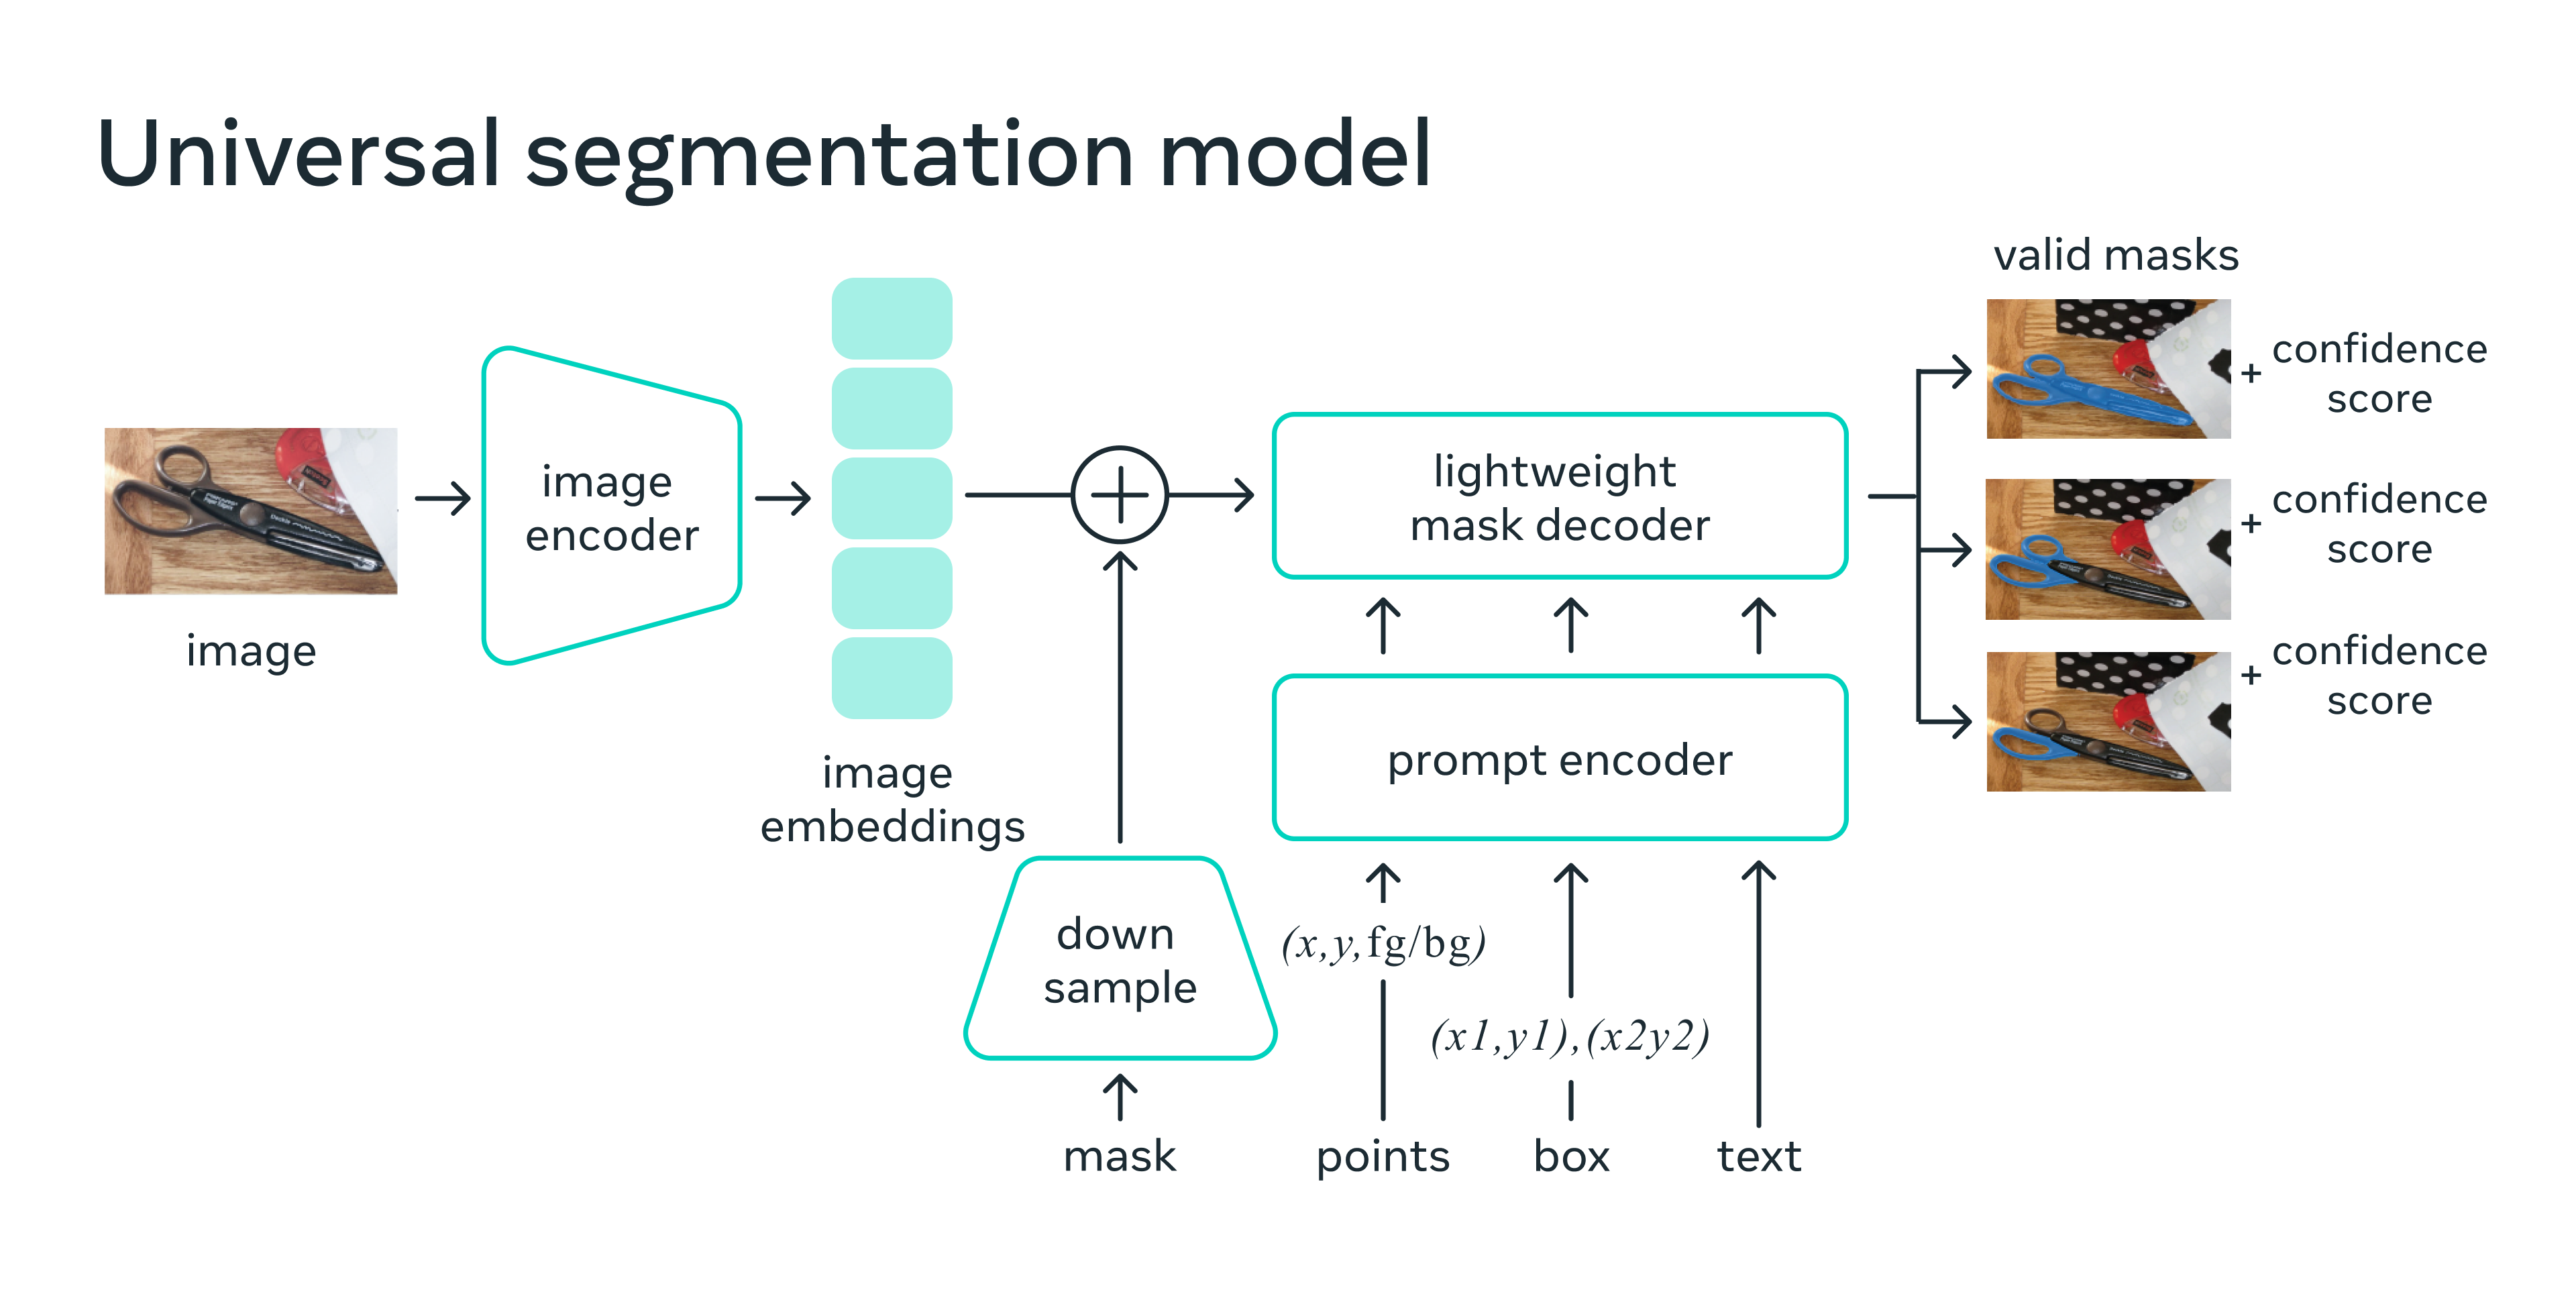
\includegraphics[width=1\linewidth]{sam_paper_dig_2.png}
    \caption{The full architecture of the Segment Anything model (SAM). Figure obtained from LugSAM paper\cite{b17}}
\end{figure}

\subsection{PeFT}

Parameter-efficient finetuning techniques were a major consideration due to the computational requirements of working with large base models on consumer hardware. We empirically evaluate 2 recently proposed techniques: LoRA \cite{b18} and $(IA)^3$ \cite{b19}. 

Such methods take advantage of the fact that pretrained models have a low "intrinsic dimension" \cite{b18} and need not operate on such high-rank representations. Thus, we can inject low-rank adapters post-training that downsample and upsample the representation, and interpolate between the adapter's output and the original weights' output at inference time. This means that we only need to train the interpolation hyperparameter ($\alpha$) and the adapter weights, while keeping the original model weights frozen.\\

This can be neatly summarized in the LoRA equation:
$$
    W_0 + \Delta W = W_0 + BA
$$

And we interpolate between the adapter weights and the original weights to obtain the latent representation at i\textsuperscript{th} layer:
$$
    \hat{y}_i(x) = \alpha W_0 x + (1 - \alpha) \Delta W x
$$

Where $W_0 \in \mathbb{R}^{d \times k}, B \in \mathbb{R}^{d \times r}, A \in \mathbb{R}^{r \times k}$, $\alpha$ is a trainable parmeter, $d$ and $k$ control the hidden dimension size, and rank $r << min(d, k)$.
\vspace{3.25pt}

As is evident by reducing the above equation, the only change to the weights during finetuning is determined by the linear transformation $BA$ which is significantly cheaper than backpropogating w.r.t $W_0$ due to operating at low-rank.
\vspace{3.25pt}

For both approaches, we finetune the adapters themselves as well as the normalization and bias parameters. Empirical evaluations with both $(IA)^3$ and LoRA demonstrate similar results, so we choose not to include their metrics.

\subsection{Other tricks}
We also utilize some other well-known techniques and tricks to boost performance. These include:
\\
\begin{itemize}
    \item Top-k ensembling: ($k=3$) averaging the best performing checkpoints 
    \item Learning rate schedules via cosine annealing
    \item Image augmentation such as flipping and \textit{randaug}\cite{b20}
    \item  validating \& training on the joint \em{val} and \em{train} set from both the challenge + warmup phase
\end{itemize}

\section{Results}

We evaluate the model on the union of the validation set from both the Challenge and Warmup phase of the competition. The metrics are given below (Table 1).\\
\\
For the LB score, we report the score from the public LB (challenge phase)

\begin{table}[htbp]
\centering
\caption{Metrics recorded for the final model}
\label{tab:my_label}
\begin{tabular}{ccc}
\hline
\textbf{Epoch} & \textbf{Val IoU} & \textbf{LB mIoU} \\
0 & 0.795 & - \\
1 & 0.826 & - \\
2 & 0.842 & 83.49 \\
\hline
\end{tabular}
\end{table}
\section{Conclusions}
In conclusion, our approach capitalizes on the strengths of pretrained foundation models and parameter-efficient fine-tuning to address the challenges posed by the UCC AI Quest competition. \\

By leveraging the SAM model and adopting PeFT methodology, we have developed a highly robust and adaptable solution capable of handling diverse scenarios with varying data quality in a robust, and computationally efficient manner.\\

We express gratitude to UCC for their role in organizing the competition and their dedication to advancing AI research and supporting the community.

\begin{thebibliography}{00}

\bibitem{b1} N. M. Zaitoun and M. J. Aqel, “Survey on Image Segmentation Techniques,” Procedia Computer Science, vol. 65, pp. 797–806, 2015, doi: https://doi.org/10.1016/j.procs.2015.09.027. Available: https://core.ac.uk/download/pdf/82543257.pdf.
\bibitem{b2} M. Dehghani, S. Gouws, O. Vinyals, J. Uszkoreit, and Ł. Kaiser, “Universal Transformers,” arXiv:1807.03819 [cs, stat], Mar. 2019, Available: https://arxiv.org/abs/1807.03819. [Accessed: Feb. 21, 2024].
\bibitem{b3} D. Cires¸an, U. Meier, and J. Schmidhuber, “Multi-column Deep Neural Networks for Image Classification,” 2012, Available: https://arxiv.org/pdf/1202.2745.pdf. [Accessed: Feb. 21, 2024]
\bibitem{b4} A. Krizhevsky, I. Sutskever, and G. E. Hinton, “ImageNet Classification with Deep Convolutional Neural Networks,” Neural Information Processing Systems, 2012. Available: https://papers.nips.cc/paper\_files/paper/2012/hash/c399862d3b9d6b76c8436e924a68c45b-Abstract.html.
\bibitem{b5} S. Hochreiter and J. Schmidhuber, “Long Short-Term Memory,” Neural Computation, vol. 9, no. 1, pp. 1–42, Jan. 1997, doi: https://doi.org/10.1162/neco.1997.9.1.1. Available: https://www.bioinf.jku.at/publications/older/2604.pdf. [Accessed: Feb. 22, 2024]
\bibitem{b6} R. Pascanu, T. Mikolov, and Y. Bengio, “On the difficulty of training Recurrent Neural Networks,” arXiv:1211.5063 [cs], Feb. 2013, Available: https://arxiv.org/abs/1211.5063. [Accessed: Feb. 22, 2024]
\bibitem{b7} Z. Wang and L. Wu, “Theoretical Analysis of Inductive Biases in Deep Convolutional Networks,” arXiv (Cornell University), May 2023, doi: https://doi.org/10.48550/arxiv.2305.08404
\bibitem{b8} A. Goyal and Y. Bengio, “Inductive biases for deep learning of higher-level cognition,” Proceedings of the Royal Society A: Mathematical, Physical and Engineering Sciences, vol. 478, no. 2266, Oct. 2022, doi: https://doi.org/10.1098/rspa.2021.0068
\bibitem{b9} A. Vaswani et al., “Attention Is All You Need,” arXiv.org, Jun. 12, 2017. Available: https://arxiv.org/abs/1706.03762
\bibitem{b10} C. Olsson et al., “In-context Learning and Induction Heads,” arXiv.org, Sep. 23, 2022. doi: https://doi.org/10.48550/arXiv.2209.11895. Available: https://arxiv.org/abs/2209.11895. [Accessed: Feb. 22, 2024]
\bibitem{b11} J. Kaplan et al., “Scaling Laws for Neural Language Models,” arXiv:2001.08361 [cs, stat], Jan. 2020, Available: https://arxiv.org/abs/2001.08361. [Accessed: Feb. 22, 2024]
\bibitem{b12} J. Yu, Z. Wang, V. Vasudevan, L. Yeung, M. Seyedhosseini, and Y. Wu, “CoCa: Contrastive Captioners are Image-Text Foundation Models,” arXiv:2205.01917 [cs], Jun. 2022, Available: https://arxiv.org/abs/2205.01917. [Accessed: Feb. 22, 2024]
\bibitem{b13} A. Dosovitskiy et al., “An Image is Worth 16x16 Words: Transformers for Image Recognition at Scale,” arXiv:2010.11929 [cs], Feb. 2024.
\bibitem{b14} A. Kirillov et al., “Segment Anything,” arXiv:2304.02643 [cs], Apr. 2023, Available: https://arxiv.org/abs/2304.02643. [Accessed: Feb. 22, 2024]
\bibitem{b15} S. Khan, M. Naseer, M. Hayat, S. W. Zamir, F. S. Khan, and M. Shah, “Transformers in Vision: A Survey,” arXiv:2101.01169 [cs], Feb. 2021, Available: https://arxiv.org/abs/2101.01169. [Accessed: Feb. 22, 2024]
\bibitem{b16} N. Ding et al., “Parameter-efficient fine-tuning of large-scale pre-trained language models,” Nature Machine Intelligence, Mar. 2023, doi: https://doi.org/10.1038/s42256-023-00626-4
\bibitem{b17} D. B. Ramesh, R. Iytha Sridhar, P. Upadhyaya, and R. Kamaleswaran, “Lung Grounded-SAM (LuGSAM): A Novel Framework for Integrating Text prompts to Segment Anything Model (SAM) for Segmentation Tasks of ICU Chest X-Rays,” www.techrxiv.org, Oct. 02, 2023. doi: https://doi.org/10.36227/techrxiv.24224761.v1. Available: https://papers.ssrn.com/sol3/papers.cfm?abstract\_id=4676192. [Accessed: Feb. 22, 2024]
\bibitem{b18} E. J. Hu et al., “LoRA: Low-Rank Adaptation of Large Language Models,” arXiv:2106.09685 [cs], Oct. 2021, Available: https://arxiv.org/abs/2106.09685. [Accessed: Feb. 22, 2024]
\bibitem{b19} H. Liu et al., “Few-Shot Parameter-Efficient Fine-Tuning is Better and Cheaper than In-Context Learning,” arXiv:2205.05638 [cs], Aug. 2022, Available: https://arxiv.org/abs/2205.05A638. [Accessed: Feb. 22, 2024]
\bibitem{b20} “Papers with Code - RandAugment Explained,” paperswithcode.com. Available: https://paperswithcode.com/method/randaugment. [Accessed: Feb. 22, 2024]

\end{thebibliography}
\end{document}